\documentclass[a4paper]{article}
\usepackage{verbatim}
\usepackage{linguex}
\usepackage{array}
\usepackage[pdftex]{graphicx}
\usepackage[english]{babel}
\usepackage[colorlinks=true, citecolor=black, linkcolor=black, urlcolor=blue, pdfborder={0 0 0}]{hyperref}
\usepackage[utf8x]{inputenc}
\usepackage{ucs}
\usepackage{amsmath}
\usepackage{amsfonts}
\usepackage{amssymb}
\usepackage{amsthm}
\usepackage[all]{xy}
\usepackage{parsetree}
\usepackage{avm}
%\usepackage{subfigure}
%\usepackage{natbib} apa style etc.

\newtheorem{theorem}{Theorem}[section]

\theoremstyle{definition}

\newtheorem{definition}[theorem]{Definition}

\begin{document}
\title{Using DOP for transformations}
\author{Andreas van Cranenburgh\footnote{0440949, \texttt{acranenb@science.uva.nl}} 
\and Joost Winter\footnote{9928545, \texttt{jwinter@science.uva.nl}}}
\maketitle

\begin{center}
Statistical Structure in Language Processing, \\
University of Amsterdam \\
Project report, first draft
\end{center}

\vspace{5em}

\begin{abstract}
In this paper, we investigate Data-Oriented Transformation,
based on the existing formalisms of Data-Oriented Parsing, synchronous
grammar, and the Goodman Reduction. The goal is to define and evaluate a general
formalism for learning arbitrary transformations composed of movement and insertions
based on annotated exemplars.  Parsing a sentence should result in a pair of trees
corresponding to the original and a transformed sentence. 
This stochastic approach contrasts with purely rule-based formalisms such as
transformational grammar, in which abstract representations are manipulated
with {\em a priori} specified operations. %The acquisition [... forgot my train of thought here; something about it being a contentious issue, structure dependency etc.]
The test case will be declarative versus interrogative sentences.
\end{abstract}

\newpage
\tableofcontents

\section{Introduction}

Data Oriented Parsing (DOP) has proven to be a successful framework for the
parsing of natural language and several other applications in computational
linguistics. In this paper, we will explore options of using a DOP-based method
to be able to perform frequently occurring transformations in natural language.
The main example used of such transformations will be that between declarative
and interrogative sentences in English, but the developed framework should be
generalizable to other transformations, such as:

\begin{itemize}
\item Transformations between affirmative and negative sentences.
\item The transformation between the `main clause' and `auxiliary clause'
	sentence order in Dutch.
\item Active versus passive sentences, focus, wh-fronting, etc.
%\item Similar transformations in other languages.
\end{itemize}

For this project, we make use of a number of existing frameworks that may prove
useful to us. In particular, these include:

\begin{itemize}
\item Synchronous grammars, as developed by David Chiang in \cite{Ch}.
\item Data Oriented Translation framework by Arjen Poutsma in \cite{Po} and
	\cite{Po2}.
\item The Goodman-reduction, as developed by Joshua Goodman in \cite{Go}.
\end{itemize}

In section \ref{sec:theor}, these underlying frameworks (as well as their
relevance to our project) will be explained in a somewhat more detailed
fashioned; then in section \ref{sec:approach}, our own approach will be
described more comprehensively; in section \ref{sec:implem}, further details
regarding our implementation will be given, and in section \ref{sec:eval}, the
obtained results will be presented.

\section{Theoretical framework}
\label{sec:theor}

We will use a data-oriented approach. This is opposed to the abstract, rule-based
formalisms such as transformational grammar, which assume abstract structures in
addition to surface structures. See figure \ref{synchdop} for a diagrammatic overview
the relation of our project to traditional, generative approach.

\begin{figure}
\centering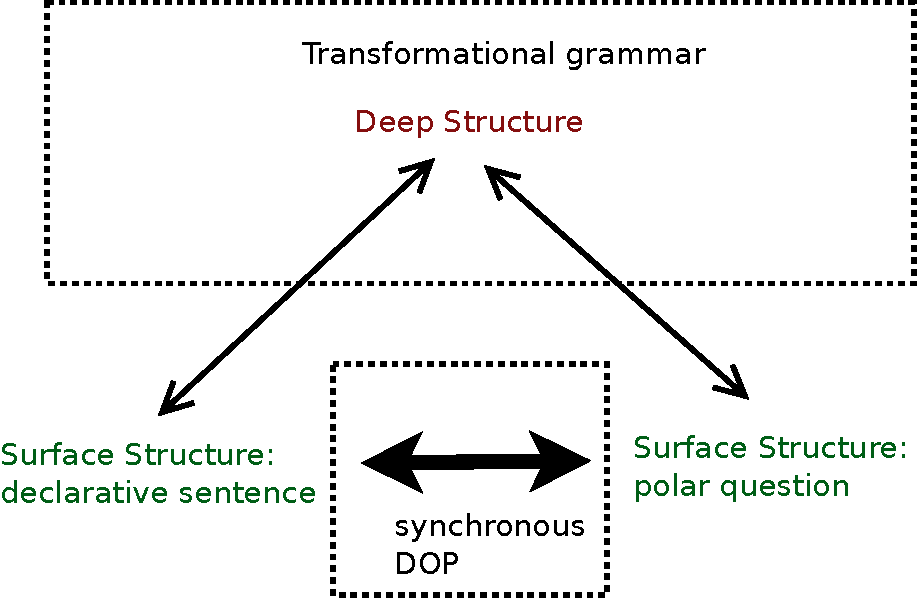
\includegraphics[width=0.7\textwidth]{synchdop-crop}
\label{synchdop}
\caption{Overview of transformations: the orthodox approach (transformational grammar),
	contrasted with our data-oriented approach}
\end{figure}

\subsection{Synchronous grammars}
\label{subsec:synch}

In \cite{Ch}, the concept of a synchronous grammar is introduced, as a tool to
easily extend the notion of a (P)CFG into the domains of translation and
transformation. The main idea, here, is that instead of single CFG-rules with a
left and right hand side, every rule now has a pair of right-hand sides -- one
corresponding to the source language, and the other corresponding to the target
language. Moreover, there has to be a bijective function between the
nonterminal symbols on both right-hand sides.

Parsing and translating using synchronous grammars is just as easy as it is for
regular PCFGs: to translate, we simply parse using the right-hand sides
corresponding to the source language. By reading off the right-hand sides
corresponding to the target language, of the rules used in the derivation, the
translation is immediately obtained.

Some problems with synchronous grammars are also mentioned in \cite{Ch}. One of
these problems is that, in reality, tree structures often do not coincide
between the original language and the translated language. For example:

\ex.
\label{johnenfr}

%failed attempt to get <=> aligned in the middle vertically. oh well.
\begin{tabular}{ r m{3em} l }
\begin{parsetree}
( .S.
	( .NP. `John' )
	( .VP.
		( .V. `misses' )
		( .NP. `Mary' )
	)
)
\end{parsetree}
& $\iff$ &
\begin{parsetree}
( .S.
	( .NP. `Mary' )
	( .VP.
		( .V. `manque' )
		( .PP.
			( .P. `à' )
			( .NP. `John' )
		)
	)
)
\end{parsetree}
\end{tabular}
\vspace{1em}

A common analysis of \ref{johnenfr} is problematic under the original
framework of synchronous grammars, because of the mismatch in the tree
structures.

Similarly, when looking at transformations between declarative and
interrogative sentences, and basing ourselves on standard analyses of the
Stanford parser (which are based on the annotation of the Penn
treebank), we encounter the following pairs of trees:

\ex. \label{marylike}

\begin{tabular}{lll}
\begin{parsetree}
( .S.
    (.NP. (.NNP. `Mary'))
    (.VP. (.VBZ. `likes')
      (.NP. (.NNS. `cars')))
)
\end{parsetree}
& $\iff$ &
\begin{parsetree}
  (.SQ. (.VBD. `does')
    (.NP. (.NNP. `Mary'))
    (.VP. (.VB. `like')
      (.NP. (.NNS. `cars')))
    )
\end{parsetree}
\end{tabular}
\vspace{1em}

Again, we here are faced with a pair of sentences, where the tree structures
are rather different from each other.

As a solution to the problem of a mismatch, the notion of flattening is named.
In this case, several CFG-rules are collapsed into a single rule, so that the
mismatch between the trees is resolved.

\subsection{DOP for translations}

In \cite{Po} and \cite{Po2}, synchronous grammars are extended from plain
PCFGs to the DOP framework: instead of looking at rules with two right-hand
sides and a corresponding set of non-terminals, we now consider pairs
subtrees with identical top nodes, and corresponding non-terminal leaf nodes.

These linked subtrees are then combined into a bag of linked subtree pairs,
which can then be used as a grammar for translations and transformations. Just
like in the case of synchronous PCFGs, we can simply parse new sentences using
the source `side' of the grammar, and derive the corresponding target side
immediately.

Formally, in \cite{Po}, linked subtree pairs are defined as follows:

\begin{definition}
Given a pair of linked trees $\langle T_1, T_2 \rangle$, a \emph{linked subtree
pair} consists of two connected and linked subgraphs $\langle t_1, t_2 \rangle$
such that:

\begin{enumerate}
\item for every pair of linked nodes in $\langle t_1, t_2 \rangle$, it holds that
	\begin{enumerate}
	\item both nodes in $\langle t_1, t_2 \rangle$ have either zero
		daughter nodes, or
	\item both nodes have all the daughter nodes of the corresponding node
		in $\langle T_1, T_2 \rangle$
	\end{enumerate}
\item every non-linked node in either $t_1$ (or $t_2$) has all the daughter
	nodes of the corresponding node in $T_1$ (or $T_2$), and
\item both $t_1$ and $t_2$ consist of more than one node.
\end{enumerate}
\end{definition}

Then, the \emph{bag of linked subtree pairs} is defined as follows: given a
corpus of linked trees $C$, the \emph{bag of linked subtree pairs} of $C$ is
the bag in which linked subtree pairs occur exactly as often as they can be
identified in $C$.

An important contrast with the earlier synchronous grammars for PCFGs, is that
in the framework of \cite{Po}, we are not necessarily dependent on strong
similarities between the tree structures on both sides (although, ultimatlely,
a strong similarity may still be a prerequisite for good performance). This
would make translations and transformations, such as in the examples given in
section \ref{subsec:synch}, possible.

Of course, it should be noted that, in this framework, it is unlikely that
\emph{all} subtrees on the source side are linked to subtrees on the target
side: especially in the (far from unlikely) case where the total number of
subtree differs, this has to be trivially false.

A problem with the DOT model, as described in \cite{Po}, consists of the fact
that the complexity of parsing new sentences can be quite huge, as the number
of subtrees can be (at worst) exponential in the number of nodes. For standard
DOP-based parsing the Goodman reduction, which will be described in the next
section, has been found to resolve such issues: however, because we do not have
a complete set of subtrees available to use, it is impossible to use this
reduction right away. This question of finding a suitable reduction for the DOT
model as described in \cite{Po} and \cite{Po2}, will be addressed at a later
stage in this report.

\subsection{Goodman reduction}

A significant problem with DOP parsing, is the fact that the number of subtrees
that have to be included is exponential in the size of the tree. In \cite{Go},
a solution to this problem is presented, that is able to yield equivalent parse
probabilities (but not equivalent derivation probabilities) to regular DOP
parsing, while limiting the number of rules to a number that is linear in the
number of tree nodes.

Here, the subtrees are replaced by a set of PCFG-rules, where nodes can be
either `addressed' or `non-addressed': in every tree, every node has a unique
address, and the addressed nodes only match with that specific address, whereas
the non-addressed nodes match with any node of the type.

It is proven in \cite{Go} that the PCFG resulting from the Goodman reduction
leads to equivalent parse probabilities as the underlying STSG:

\begin{theorem}
This construction [the Goodman-reduction] produces PCFG trees homomorphic to
the STSG trees with equal probability.
\end{theorem}

\section{Approach}
\label{sec:approach}

\subsection{Definition of DOP model}

We will assume a parallel corpus of pairs of trees with declarative and
interrogative versions of sentences. This assumption lies on the extreme
end of supervised parsing; other options are a bag of unrelated sentences
marked as declarative or interrogative in their root node. Whether the
assumption of a parallel corpus is cognitively plausible in terms of
language acquisition is irrelevant because the point is to learn
transformations from exemplars alone, without relying on built in primitives
for movement and insertions, or on a common, abstract representation for
sentences such as Deep Structures or Logical Form in generative grammar.

Assuming ordered pairs of trees, $\langle T_{\mathit{s}},
T_{\mathit{t}} \rangle $, may be enough to learn transformations
from data alone. Naturally the word forms will often coincide, so words are
implicitly linked (although this may be problematic with multiple occurrences
in the same sentence). Further annotation could add indices for each
constituent, but this implies labor-intensive annotation. More difficult than
the linking problem is the problem of structure mismatch. Consider the following
example:

\ex. \label{maryhappy}

\begin{tabular}{lll}
\begin{parsetree}
( .S.
    (.NP. (.NNP. `Mary'))
    (.VP. (.VBZ. `is')
      (.ADJP. (.JJ. `happy')))
)
\end{parsetree}
& $\iff$ &
\begin{parsetree}
  (.SQ. 
    (.VBZ. `is')
    (.NP. (.NNP. `Mary'))
    (.ADJP. (.JJ. `happy'))
    )
\end{parsetree}
\end{tabular}
\vspace{1em}

In the phrase-structure annotation of the interrogative of \ref{maryhappy} (as produced
by the Stanford parser), the \textsc{VP} constituent has arguably become a
discontinuous constituent \cite{Ha}, but due to a strong, pragmatically
motivated preference for orthodox phrase-structures in computational linguistics (as
well as a completely indefensible Anglocentrism), such
information is sacrificed by collapsing the phrase-structure. This means that
the phrase-structure no longer encodes the connection of the verb and its
direct object. A more elaborate representation such as employed in the discontinuous
constituent phrase-structure grammar of \cite{Ha} would make it possible to streamline
the annotation of sentences so that less configurational information can be preserved.
Note that discontinuous constituents are only a minor step in the spectrum of
constituency versus dependency. While a discontinuous constituent violates the
canonical definition of a tree, it is still word order which determines constituency
(e.g., in the example a fronted auxiliary verb signifies VSO order),
and it is not obvious that a free word-order language could be profitably
described by such a representation. When \ref{maryhappy} is represented using
discontinuous constituents, the tree could look like this:

\ex. \label{marydiscont}

\begin{center}
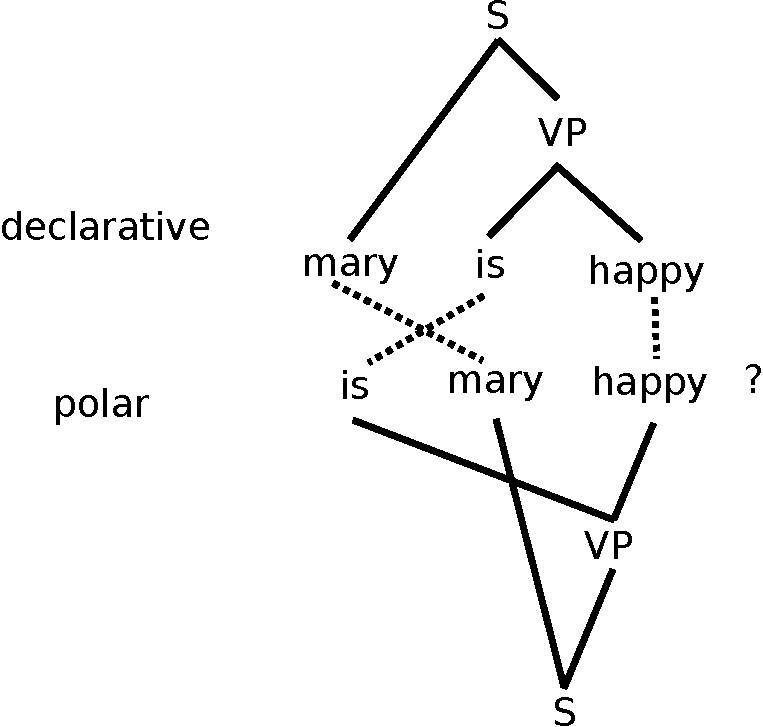
\includegraphics[width=0.5\textwidth]{maryishappy-crop.pdf}
\end{center}
\vspace{1em}

It is clear that this kind of representation provides a way to avoid structure
mismatch as a result of movement completely (ie., the bag of non-terminals will
be equivalent for both structures). The absence of the auxiliary `did' in the
declarative such as in \ref{marylike} can be represented by trace elements; an
even simpler strategy would be to allow structure mismatch as long as one of
the trees is a proper subtree of the other. The reason that it may be
worthwhile to avoid structure mismatch is that it maximizes the number of
parallel subtrees, which minimizes the violation of the DOP hypothesis stating
that all fragments should count in order to fully exploit the data at hand. It
may turn out that without isomorphic phrase-structures, the generalizing power
of synchronous DOP is not sufficient to handle complex, novel sentences (long
constituents, relative or embedded clauses, etc.).

The same definition for subtrees and fragments can be applied to discontinuous
structures, it is basically a matter of annotation and implementation to employ
them, not formalism.  Whether it will be necessary or worthwhile to adopt
discontinuous constituents will have to be determined emprically. Initially we
will attempt to use the standard PTB phrase-structure annotation and see how well
it works; this has the obvious advantage of the availability of large corpora such
as the WSJ, which can complement a small, hand-annotated parallel treebank.

\newpage %fixme

As a compromise between the impoverished PTB annotation and the rich but non-standard
discontinuous annotation, we could consider labelling POS tags with (former) parent
annotations, e.g.:

\ex. \label{maryhappyann}

\begin{tabular}{lll}
\begin{parsetree}
( .S.
    (.NP. (.NNP. `Mary'))
    (.VP. (.VBZ. `is')
      (.ADJP. (.JJ. `happy')))
)
\end{parsetree}
& $\iff$ &
\begin{parsetree}
  (.SQ.
    (.VBZ[VP]. `is')
    (.NP. 
	(.NNP. `Mary'))
    (.ADJP[VP]. (.JJ. `happy'))
    )
\end{parsetree}
\end{tabular}
\vspace{1em}

As operations we will restrict ourselves to the standard substitution operation. While
it may seem obvious to extend the DOP framework with movement and adjunction operations,
that has the downside of having to adapt the existing, well-defined formalisms,
including their probability models. On top of that we set out to induce transformations
from data alone, so making such things part of the formalism means smuggling in
{\em a priori} expectations (albeit only in a very general sense).

As estimation method we will employ the standard DOP1 estimator, but DOP* or %cite these
backoff-DOP can be considered as well. Although sparsity of evidence is
claimed to be an insurmountable problem for non-nativist theories by
generativists, for example the transformation of aux-fronting seems simple
enough given elaborate information such as phrase structures. For this reason
it would seem that DOP1 should be adequate.

\subsection{A reduction for synchronous DOP}

As an instantiation of the previously mentioned assumptions, we will apply
Data-Oriented Translation to transformations. For implementation efficiency
we would like to use the Goodman reduction.

We are now faced with the situation, that we cannot simply apply the Goodman
reduction, reducing subtree pairs to PCFG rules, because of the reason that not
every subtree will always be a part of a subtree pair. In particular, the
PCFG-rules themselves, the `building blocks' of the Goodman reduction, may not
be a part of a subtree pair. This leads us to wonder whether it is possible to,
in some way or another, still perform a Goodman-like reduction on the bag of
linked subtree pairs.

It turns out that, indeed, a reduction is possible over the bag of linked
subtree pairs. For this, consider the notion of a \emph{minimal linked subtree
pair}:

\begin{definition}
For a pair of linked trees $\langle T_1, T_2 \rangle$, a \emph{minimal linked
subtree pair} is a linked subtree pair $\langle t_1, t_2 \rangle$, s.t. $t_1
\subseteq T_1$, $t_2 \subseteq T_2$, such that there is no other linked pair
$\langle s_1, s_2 \rangle$ where $s_1 \subsetneq t_1$ and $s_2 \subsetneq t_2$.
\end{definition}

\begin{theorem}
Every pair of linked trees can be reconstructed from the minimal linked subtree
pairs derived from it.
\end{theorem}

\begin{proof}

Assume that there is a pair of linked trees $\langle T_1, T_2 \rangle$ for
which this is not possible, given a certain bag of linked subtree pairs. Then
there has to be some linked pair of subtrees $\langle t_1, t_2 \rangle$ for
which:

\begin{enumerate}
\item It is not possible to construct $\langle t_1, t_2 \rangle$ from minimal
	linked subtree pairs.
\item All pairs of subtrees $\langle s_1, s_2 \rangle \subsetneq \langle t_1,
	t_2 \rangle$ can be constructed from minimal subtree linked pairs.
\end{enumerate}

It is impossible that this pair of subtrees is itself minimal: if it were, it
could trivially be constructed from linked minimal subtree pairs. So, for this
case to hold, the linked subtree pair $\langle t_1, t_2 \rangle$ must have a
proper subset $\langle s_1, s_2 \rangle$.

\ldots (incomplete but I know how to finish)

\end{proof}

In other words: just like the PCFG rules can be used as the `building blocks'
for the Goodman reduction, the minimal linked subtree pairs as defined above
can be used as the `building blocks' for a similar reduction. It should be
noted that, for all means and purposes, such minimal subtrees can be worked
with, as if they were simple CFG-rules, that just happen to have an additional
internal structure (which is ignored by the parser).

Like in the Goodman-reduction, we replace every elementary tree (i.e. every
minimal linked subtree pair) with $2^{(k+1)}$ new rules, where $k$ is the
number of nonterminals occurring as leaf nodes (which has to be equal on the
left and right hand sides). For the root node, and for every nonterminal node,
either an `addressed' version or a `non-addressed' version can occur.

\begin{theorem}
A `Goodman-like' reduction based on minimal linked subtree pairs leads to
equivalent parse probabilities (but not equivalent derivation probabilities) as
the original synchronous DOP model.
\end{theorem}

\section{Implementation}
\label{sec:implem}

TBD.

\section{Evaluation}
\label{sec:eval}

Standard \textsc{parseval} measures (with \texttt{EVALB}), transformations in both
directions. Take (part of) WSJ treebank, hand annotate corresponding transformed
sentences.

TBD. 

\section{Conclusions}

TBD.

\label{sec:conc}

%todo bibtex this. natbib, APA style.

\begin{thebibliography}{BlAbLa00}

%todo: add URLs with \url{http://...}, complete references
\bibitem[Ch]{Ch} Chiang, David (20XX), ``An Introduction to Synchronous Grammars.''

\bibitem[Po]{Po} Poutsma, Arjen (2000), ``Data-Oriented Translation,'' presented at
	COLING 2000.

\bibitem[Po2]{Po2} Poutsma, Arjen (2000), ``Data-Oriented Translation,'' master's
	thesis, University of Amsterdam.

\bibitem[Go]{Go} Goodman, Joshua (2002), ``Efficient Parsing of DOP with
	PCFG-reductions'' in \emph{Data Oriented Parsing} (2002), Bod, Rens;
	Sima'an, Khalil; and Scha, Remko, eds.

\bibitem[Ha]{Ha} Harman, Gilbert H.\ (1963), ``Generative Grammars without
	Transformation Rules: A Defense of Phrase-Structure,'' \emph{Language},
	vol.\ 39, no.\ 4, pp.\ 597-616

%This reference has sections on learning aux-fronting from positive data alone:
%\bibitem[Ma]{Ma} MacWhinney, Brian (20XX), ``A multiple process solution to the logical
%problem of language acquisition'' [...]

%This reference should have some experiments with childes data to parse
%interrogatives based on declaratives etc.
%\bibitem[Bo]{Bo} Bod, Rense. A linguistic investigation into unsupervised DOP

\end{thebibliography}

\end{document}

comments & todo items go here . . .

typesetting discontinuous constituent trees:

http://www.ling.uni-potsdam.de/~rvogel/xyling
Ralf Vogel's xyling package: this package is very flexible and powerful, and does not use pstricks etc. (so you can see the trees in the dvi output). It supports labeling of branches as well as nodes, as well as lines and arrows that relate discontinuous pieces of the tree. [package, documentation]

http://tug.ctan.org/tex-archive/macros/latex/contrib/rrgtrees/
the RRGtrees package, by David Gardner, provides LaTeX macros for the sorts of
tree diagram used in Role and Reference Grammar. This includes trees with
crossing lines, as is required by some languages in this theory. It uses
pstricks. [The distribution includes a `make' file (so, just `make
rrgtrees.sty' will create the style file), but if you haven't got `make' you
can create rrgtrees.sty by running latex over rrgtrees.ins.]

